\documentclass[11pt,a4paper]{article}
\usepackage[hyperref]{naaclhlt2019}
\usepackage{times}
\usepackage{latexsym}
\usepackage{xspace}
\usepackage{multirow}
\usepackage{url}
\usepackage{booktabs}
\usepackage{tikz,tikz-qtree}
\usepackage{pgfplots}
\usepackage{amssymb}
\usepackage{xfrac}
\usepackage{graphicx}
\usepackage{tablefootnote}
\usepackage{amsmath}
\usepackage{enumitem}
\pgfplotsset{compat=1.14}

\newcommand\BibTeX{B{\sc ib}\TeX}
\newcommand\bert{BERT\xspace}

\aclfinalcopy % comment this when submitting the paper
%\def\aclpaperid{***} %  Enter the acl Paper ID here

%\setlength\titlebox{5cm}
% You can expand the titlebox if you need extra space
% to show all the authors. Please do not make the titlebox
% smaller than 5cm (the original size); we will check this
% in the camera-ready version and ask you to change it back.

\hyphenation{OpenAI}

\definecolor{g-red}{HTML}{DB4437}
\definecolor{g-blue}{HTML}{4285F4}
\definecolor{g-green}{HTML}{0F9D58}
\definecolor{g-yellow}{HTML}{F4B400}
\definecolor{g-orange}{HTML}{FF9800}
\definecolor{g-grey}{HTML}{9E9E9E}

\setlength{\tabcolsep}{0.3em}

\usepackage{todonotes}


\newcounter{mw}
\newcommand{\mw}[1]{%
\refstepcounter{mw}%
{%
\todo[color=orange, size=\footnotesize]{%
[\textbf{mw:\themw}] #1}%
}}%

\newcounter{jd}
\newcommand{\jd}[1]{%
\refstepcounter{jd}%
{%
\todo[color=green, size=\footnotesize]{%
[\textbf{jd:\thekt}] #1}%
}}%

\newcounter{kl}
\newcommand{\kl}[1]{%
\refstepcounter{kl}%
{%
\todo[color=magenta, size=\footnotesize]{%
[\textbf{kl:\thekl}] #1}%
}}%

\newcommand\bertbase{BERT$_{\small \textsc{BASE}}$\xspace}
\newcommand\bertlarge{BERT$_{\small \textsc{LARGE}}$\xspace}

\title{\textbf{BERT}: Pre-training of Deep Bidirectional Transformers for \\ Language Understanding}

\author{Jacob Devlin \quad Ming-Wei Chang \quad Kenton Lee \quad Kristina Toutanova \\
  Google AI Language \\
  {\tt \{jacobdevlin,mingweichang,kentonl,kristout\}@google.com} \\}

\date{}

% REMOVE THIS IN THE FINAL COPY!
% \hypersetup{draft}

\begin{document}
\maketitle
\begin{abstract}
  We introduce a new language representation model called {\bf \bert}, which stands for \textbf{B}idirectional \textbf{E}ncoder \textbf{R}epresentations from \textbf{T}ransformers. Unlike recent language representation models~\cite{peters-etal:2018:_deep, radford-etal:2018},  \bert is designed to pre-train deep bidirectional representations by jointly conditioning on both left and right context in all layers. As a result, the pre-trained \bert representations can be fine-tuned with just one additional output layer to create state-of-the-art models for a wide range of tasks, such as question answering and language inference, {\em without} substantial task-specific architecture modifications.

\bert is conceptually simple and empirically powerful. It obtains new state-of-the-art results on eleven natural language processing tasks, including pushing the GLUE benchmark to {\bf 80.4\%} ({\bf 7.6}\% absolute improvement), MultiNLI accuracy to {\bf 86.7\%} ({\bf 5.6}\% absolute improvement) and the SQuAD v1.1 question answering Test F1 to {\bf 93.2} ({\bf 1.5} absolute improvement), outperforming human performance by {\bf 2.0}.

\end{abstract}

\section{Introduction}

Language model pre-training has shown to be effective for improving many natural language processing tasks~\cite{dai-le:2015:_semi,peters-etal:2017:_semi, peters-etal:2018:_deep, radford-etal:2018, howard-ruder:2018}. These tasks include sentence-level tasks such as natural language inference~\cite{bowman-etal:2015, williams-nangia-bowman:2018} and paraphrasing~\cite{dolan-brockett:2005:_autom}, which aim to predict the relationships between sentences by analyzing them holistically, as well as token-level tasks such as named entity recognition~\cite{tjong-de:2003} and SQuAD question answering~\cite{rajpurkar-etal:2016:_squad}, where models are required to produce fine-grained output at the token-level.

There are two existing strategies for applying pre-trained language representations to downstream tasks: {\em feature-based} and {\em fine-tuning}. The feature-based approach, such as ELMo~\cite{peters-etal:2018:_deep}, uses tasks-specific architectures that include the pre-trained representations as additional features. The fine-tuning approach, such as the Generative Pre-trained Transformer (OpenAI GPT)~\cite{radford-etal:2018}, introduces minimal task-specific parameters, and is trained on the downstream tasks by simply fine-tuning the pre-trained parameters. In previous work, both approaches share the same objective function during pre-training, where they use unidirectional language models to learn general language representations.

We argue that current techniques severely restrict the power of the pre-trained representations, especially for the fine-tuning approaches. The major limitation is that standard language models are unidirectional, and this limits the choice of architectures that can be used during pre-training. For example, in OpenAI GPT, the authors use a left-to-right architecture, where every token can only attended to previous tokens in the self-attention layers of the Transformer~\cite{vaswani-etal:2017:_atten}. Such restrictions are sub-optimal for sentence-level tasks, and could be devastating when applying fine-tuning based approaches to token-level tasks such as SQuAD question answering \cite{rajpurkar-etal:2016:_squad}, where it is crucial to incorporate context from both directions.

In this paper, we improve the fine-tuning based approaches by proposing \bert: \textbf{B}idirectional \textbf{E}ncoder \textbf{R}epresentations from \textbf{T}ransformers. \bert addresses the previously mentioned unidirectional constraints by proposing a new pre-training objective: the ``masked language model''~(MLM), inspired by the Cloze task~\cite{taylor:1953:_cloze}. The masked language model randomly masks some of the tokens from the input, and the objective is to predict the original vocabulary id of the masked word based only on its context. Unlike left-to-right language model pre-training, the MLM objective allows the representation to fuse the left and the right context, which allows us to pre-train a deep bidirectional Transformer. In addition to the masked language model, we also introduce a ``next sentence prediction'' task that jointly pre-trains text-pair representations.

The contributions of our paper are as follows:
\begin{itemize}
  \item We demonstrate the importance of bidirectional pre-training for language representations. Unlike \citet{radford-etal:2018}, which uses unidirectional language models for pre-training, \bert uses masked language models to enable pre-trained deep bidirectional representations. This is also in contrast to \citet{peters-etal:2018:_deep}, which uses a shallow concatenation of independently trained left-to-right and right-to-left LMs.
  \item We show that pre-trained representations eliminate the needs of many heavily-engineered task-specific architectures. \bert is the first fine-tuning based representation model that achieves state-of-the-art performance on a large suite of sentence-level {\em and} token-level tasks, outperforming many systems with task-specific architectures.
  \item \bert advances the state-of-the-art for eleven NLP tasks. We also report extensive ablations of \bert, demonstrating that the bidirectional nature of our model is the single most important new contribution. The code and pre-trained model will be available at \url{goo.gl/language/bert}.\footnote{Will be released before the end of October 2018.}
\end{itemize}


\section{Related Work}
There is a long history of pre-training general language representations, and we briefly review the most popular approaches in this section.
\subsection{Feature-based Approaches}
Learning widely applicable representations of words has been an active area of research for decades, including non-neural~\cite{brown-etal:1992:_class,ando-zhang:2005, blitzer-mcdonald-pereira:2006:_domain} and neural~\cite{collobert-weston:2008, mikolov-etal:2013, pennington-socher-manning:2014:_glove} methods. Pre-trained word embeddings are considered to be an integral part of modern NLP systems, offering significant improvements over embeddings learned from scratch~\cite{turian-ratinov-bengio:2010:_word_repres}.

These approaches have been generalized to coarser granularities, such as sentence embeddings~\cite{kiros-etal:2015:_skip, logeswaran2018an} or paragraph embeddings~\cite{le-mikolov:2014:_distr}. As with traditional word embeddings, these learned representations are also typically used as features in a downstream model.

ELMo~\cite{peters-etal:2017:_semi} generalizes traditional word embedding research along a different dimension. They propose to extract \emph{context-sensitive} features from a language model. When integrating contextual word embeddings with existing task-specific architectures, ELMo advances the state-of-the-art for several major NLP benchmarks~\cite{peters-etal:2018:_deep} including question answering~\cite{rajpurkar-etal:2016:_squad} on SQuAD, sentiment analysis~\cite{socher-etal:2013:_recur}, and named entity recognition~\cite{tjong-de:2003}.

\subsection{Fine-tuning Approaches}
A recent trend in transfer learning from language models (LMs) is to pre-train some model architecture on a LM objective before fine-tuning that same model for a supervised downstream task~\cite{dai-le:2015:_semi, howard-ruder:2018, radford-etal:2018}. The advantage of these approaches is that few parameters need to be learned from scratch. At least partly due this advantage, OpenAI GPT~\cite{radford-etal:2018} achieved previously state-of-the-art results on many sentence-level tasks from the GLUE benchmark~\cite{wang-etal:2018:_glue}.

\begin{figure*}[t]
\begin{center}
\includegraphics[width=\textwidth]{figures/BERT_comparisons.pdf}
\end{center}
\caption{Differences in pre-training model architectures. BERT uses a bidirectional Transformer. OpenAI GPT uses a left-to-right Transformer. ELMo uses the concatenation of independently trained left-to-right and right-to-left LSTM to generate features for downstream tasks. Among three, only \bert representations are jointly conditioned on both left and right context in all layers.}
\label{fig:BERT_comparisons}
\end{figure*}

\subsection{Transfer Learning from Supervised Data}
While the advantage of unsupervised pre-training is that there is a nearly unlimited amount of data available, there has also been work showing effective transfer from supervised tasks with large datasets, such as natural language inference~\cite{conneau-EtAl:2017:EMNLP2017} and machine translation~\cite{mccann-etal:2017:_learn_trans}. Outside of NLP, computer vision research has also demonstrated the importance of transfer learning from large pre-trained models, where an effective recipe is to fine-tune models pre-trained on ImageNet~\cite{imagenet_cvpr09, yosinski2014transferable}. 


\section{BERT}
\label{sec:bert}

We introduce BERT and  its detailed implementation in this section. We first cover the model architecture and the input representation for BERT. We then introduce the pre-training tasks, the core innovation in this paper, in Section~\ref{sec:pretraining_tasks}. The pre-training procedures, and fine-tuning procedures are detailed in Section~\ref{sec:pretraining_procedure} and~\ref{sec:finetuning_procedure}, respectively. Finally, the differences between BERT and OpenAI GPT are discussed in Section~\ref{sec:comparing_bert_and_openai}.

\subsection{Model Architecture}
\label{sec:model_architecture}

BERT's model architecture is a multi-layer bidirectional Transformer encoder based on the original implementation described in \citet{vaswani-etal:2017:_atten} and released in the {\tt tensor2tensor} library.\footnote{https://github.com/tensorflow/tensor2tensor} Because the use of Transformers has become ubiquitous recently and our implementation is effectively identical to the original, we will omit an exhaustive background description of the model architecture and refer readers to \citet{vaswani-etal:2017:_atten} as well as excellent guides such as ``The Annotated Transformer.''\footnote{http://nlp.seas.harvard.edu/2018/04/03/attention.html}

In this work, we denote the number of layers (i.e., Transformer blocks) as $L$, the hidden size as $H$, and the number of self-attention heads as $A$. In all cases we set the feed-forward/filter size to be $4H$, i.e., 3072 for the $H=768$ and 4096 for the $H=1024$. We primarily report results on two model sizes:

\begin{itemize}
\item {\bf \bertbase}: L=12, H=768, A=12, Total Parameters=110M
\item {\bf \bertlarge}: L=24, H=1024, A=16, Total Parameters=340M
\end{itemize}

\bertbase was chosen to have an identical model size as OpenAI GPT for comparison purposes. Critically, however, the BERT Transformer uses bidirectional self-attention, while the GPT Transformer uses constrained self-attention where every token can only attend to context to its left. We note that in the literature the bidirectional Transformer is often referred to as a ``Transformer encoder'' while the left-context-only version is referred to as a ``Transformer decoder'' since it can be used for text generation. The comparisons between BERT, OpenAI GPT and ELMo are shown visually in Figure~\ref{fig:BERT_comparisons}.


\subsection{Input Representation}
\label{sec:input_representation}


\begin{figure*}[tbh]
\begin{center}
\hspace{-0.2in}
\includegraphics[width=400px]{figures/Input_Emebeddings.pdf}
\end{center}
\caption{BERT input representation. The input embeddings is the sum of the token embeddings, the segmentation embeddings and the position embeddings.}
\label{tab:input_emebeddings}
\end{figure*}

Our input representation is able to unambiguously represent both a single text sentence or a pair of text sentences (e.g., [Question, Answer]) in one token sequence.\footnote{Throughout this work, a ``sentence'' can be an arbitrary span of contiguous text, rather than an actual linguistic sentence. A ``sequence'' refers to the input token sequence to BERT, which may be a single sentence or two sentences packed together.} For a given token, its input representation is constructed by summing the corresponding token, segment and position embeddings. A visual representation of our input representation is given in Figure~\ref{tab:input_emebeddings}. 

The specifics are:

\begin{itemize} 
\item We use WordPiece embeddings \cite{wu-etal:2016:_googl} with a 30,000 token vocabulary. We denote split word pieces with {\tt \#\#}.
\item We use learned positional embeddings with supported sequence lengths up to 512 tokens.
\item The first token of every sequence is always the special classification embedding ({\tt [CLS]}). The final hidden state (i.e., output of Transformer) corresponding to this token is used as the aggregate sequence representation for classification tasks. For non-classification tasks, this vector is ignored.
\item Sentence pairs are packed together into a single sequence. We differentiate the sentences in two ways. First, we separate them with a special token ({\tt [SEP]}). Second, we add a learned sentence {\tt A} embedding to every token of the first sentence and a sentence {\tt B} embedding to every token of the second sentence.
\item For single-sentence inputs we only use the sentence {\tt A} embeddings.
\end{itemize}

\subsection{Pre-training Tasks}
\label{sec:pretraining_tasks}

Unlike \citet{peters-etal:2018:_deep} and \citet{radford-etal:2018}, we do not use traditional left-to-right or right-to-left language models to pre-train BERT. Instead, we pre-train BERT using two novel unsupervised prediction tasks, described in this section.

\subsubsection{Task \#1: Masked LM}
Intuitively, it is reasonable to believe that a deep bidirectional model is strictly more powerful than either a left-to-right model or the shallow concatenation of a left-to-right and right-to-left model. Unfortunately, standard conditional language models can only be trained left-to-right {\it or} right-to-left, since bidirectional conditioning would allow each word to indirectly ``see itself'' in a multi-layered context.

In order to train a deep bidirectional representation, we take a straightforward approach of masking some percentage of the input tokens at random, and then predicting only those masked tokens. We refer to this procedure as a ``masked LM'' (MLM), although it is often referred to as a {\it Cloze} task in the literature~\cite{taylor:1953:_cloze}. In this case, the final hidden vectors corresponding to the mask tokens are fed into an output softmax over the vocabulary, as in a standard LM. In all of our experiments, we mask 15\% of all WordPiece tokens in each sequence at random. In contrast to denoising auto-encoders \cite{vincent:2008}, we only predict the masked words rather than reconstructing the entire input.

Although this does allow us to obtain a bidirectional pre-trained model, there are two downsides to such an approach. The first is that we are creating a mismatch between pre-training and fine-tuning, since the {\tt [MASK]} token is never seen during fine-tuning. To mitigate this, we do not always replace ``masked'' words with the actual {\tt [MASK]} token. Instead, the training data generator chooses 15\% of tokens at random, e.g., in the sentence {\tt {\small my dog is hairy}} it chooses {\tt {\small hairy}}. It then performs the following procedure:
\begin{itemize}
\item Rather than {\em always} replacing the chosen words with {\tt [MASK]}, the data generator will do the following:
\item 80\% of the time: Replace the word with the {\tt [MASK]} token, e.g., {\tt {\small my dog is hairy $\rightarrow$ my dog is [MASK]}}
\item 10\% of the time: Replace the word with a random word, e.g., {\tt {\small my dog is hairy $\rightarrow$ my dog is apple}}
\item 10\% of the time: Keep the word unchanged, e.g., {\tt {\small my dog is hairy $\rightarrow$ my dog is hairy}}. The purpose of this is to bias the representation towards the actual observed word.
\end{itemize}

The Transformer encoder does not know which words it will be asked to predict or which have been replaced by random words, so it is forced to keep a distributional contextual representation of {\it every} input token. Additionally, because random replacement only occurs for 1.5\% of all tokens (i.e., 10\% of 15\%), this does not seem to harm the model's language understanding capability. 

The second downside of using an MLM is that only 15\% of tokens are predicted in each batch, which suggests that more pre-training steps may be required for the model to converge. In Section~\ref{sec:num_training_steps} we demonstrate that MLM does converge marginally slower than a left-to-right model (which predicts every token), but the empirical improvements of the MLM model far outweigh the increased training cost.

\subsubsection{Task \#2: Next Sentence Prediction}
Many important downstream tasks such as Question Answering (QA) and Natural Language Inference (NLI) are based on understanding the {\it relationship} between two text sentences, which is not directly captured by language modeling. In order to train a model that understands sentence relationships, we pre-train a binarized {\it next sentence prediction} task that can be trivially generated from any monolingual corpus. Specifically, when choosing the sentences {\tt A} and {\tt B} for each pre-training example, 50\% of the time {\tt B} is the actual next sentence that follows {\tt A}, and 50\% of the time it is a random sentence from the corpus. For example:
\begin{align*}
\text{Input\;} &= \text{\tt {\scriptsize [CLS] the man went to [MASK] store [SEP]}} \\ 
& \text{\tt {\scriptsize \;\;\;\;\;\;\;he bought a gallon [MASK] milk [SEP]}}\\
\text{Label} &= \text{\tt {\scriptsize IsNext}} \\
\\
\text{Input\;} &= \text{\tt {\scriptsize [CLS] the man [MASK] to the store [SEP]}}\\
&\text{\tt {\scriptsize \;\;\;\;\;\;\;penguin [MASK] are flight \#\#less birds [SEP]}}\\
\text{Label} &= \text{\tt {\scriptsize NotNext}}
\end{align*}
We choose the {\tt {\small NotNext}} sentences completely at random, and the final pre-trained model achieves 97\%-98\% accuracy at this task. Despite its simplicity, we demonstrate in Section~\ref{sec:task_ablation} that pre-training towards this task is very beneficial to both QA and NLI.

\subsection{Pre-training Procedure}
\label{sec:pretraining_procedure}

The pre-training procedure largely follows the existing literature on language model pre-training. For the pre-training corpus we use the concatenation of BooksCorpus (800M words) \cite{zhu:2015} and English Wikipedia (2,500M words). For Wikipedia we extract only the text passages and ignore lists, tables, and headers. It is critical to use a document-level corpus rather than a shuffled sentence-level corpus such as the Billion Word Benchmark \cite{chelba-etal:2013:_one} in order to extract long contiguous sequences.

To generate each training input sequence, we sample two spans of text from the corpus, which we refer to as ``sentences'' even though they are typically much longer than single sentences (but can be shorter also). The first sentence receives the {\tt A} embedding and the second receives the {\tt B} embedding. 50\% of the time {\tt B} is the actual next sentence that follows {\tt A} and 50\% of the time it is a random sentence, which is done for the ``next sentence prediction'' task. They are sampled such that the combined length is $\le$ 512 tokens. The LM masking is applied after WordPiece tokenization with a uniform masking rate of 15\%, and no special consideration given to partial word pieces.

We train with batch size of 256 sequences (256 sequences * 512 tokens = 128,000 tokens/batch) for 1,000,000 steps, which is approximately 40 epochs over the 3.3 billion word corpus. We use Adam with learning rate of 1e-4, ${\beta}_1=0.9$, ${\beta}_2=0.999$, L2 weight decay of $0.01$, learning rate warmup over the first 10,000 steps, and linear decay of the learning rate. We use a dropout probability of 0.1 on all layers. We use a {\tt gelu} activation \cite{hendrycks:2016} rather than the standard {\tt relu}, following OpenAI GPT. The training loss is the sum of the mean masked LM likelihood and mean next sentence prediction likelihood.

Training of \bertbase was performed on 4 Cloud TPUs in Pod configuration (16 TPU chips total).\footnote{https://cloudplatform.googleblog.com/2018/06/Cloud-TPU-now-offers-preemptible-pricing-and-global-availability.html} Training of \bertlarge was performed on 16 Cloud TPUs (64 TPU chips total). Each pre-training took 4 days to complete.

\subsection{Fine-tuning Procedure}
\label{sec:finetuning_procedure}

For sequence-level classification tasks, BERT fine-tuning is straightforward. In order to obtain a fixed-dimensional pooled representation of the input sequence, we take the final hidden state (i.e., the output of the Transformer) for the first token in the input, which by construction corresponds to the the special {\tt [CLS]} word embedding. We denote this vector as $C \in \mathbb{R}^{H}$. The only new parameters added during fine-tuning are for a classification layer $W \in \mathbb{R}^{K \times H}$, where $K$ is the number of classifier labels. The label probabilities $P \in \mathbb{R}^{K}$ are computed with a standard softmax, $P = {\rm softmax}(CW^T)$. All of the parameters of BERT and $W$ are fine-tuned jointly to maximize the log-probability of the correct label. For span-level and token-level prediction tasks, the above procedure must be modified slightly in a task-specific manner. Details are given in the corresponding subsection of Section~\ref{sec:experiments}.

For fine-tuning, most model hyperparameters are the same as in pre-training, with the exception of the batch size, learning rate, and number of training epochs. The dropout probability was always kept at 0.1. The optimal hyperparameter values are task-specific, but we found the following range of possible values to work well across all tasks:

\begin{itemize}[noitemsep]
\item {\bf Batch size}: 16, 32
\item {\bf Learning rate (Adam)}: 5e-5, 3e-5, 2e-5
\item {\bf Number of epochs}: 3, 4
\end{itemize}

We also observed that large data sets (e.g., 100k+ labeled training examples) were far less sensitive to hyperparameter choice than small data sets. Fine-tuning is typically very fast, so it is reasonable to simply run an exhaustive search over the above parameters and choose the model that performs best on the development set.

\subsection{Comparison of BERT and OpenAI GPT}
\label{sec:comparing_bert_and_openai}

The most comparable existing pre-training method to BERT is OpenAI GPT, which trains a left-to-right Transformer LM on a large text corpus. In fact, many of the design decisions in BERT were intentionally chosen to be as close to GPT as possible so that the two methods could be minimally compared. The core argument of this work is that the two novel pre-training tasks presented in Section~\ref{sec:pretraining_tasks} account for the majority of the empirical improvements, but we do note that there are several other differences between how BERT and GPT were trained:

\begin{itemize}
\item GPT is trained on the BooksCorpus (800M words); BERT is trained on the BooksCorpus (800M words) and Wikipedia (2,500M words).
\item GPT uses a sentence separator ({\tt [SEP]}) and classifier token ({\tt [CLS]}) which are only introduced at fine-tuning time; BERT learns {\tt [SEP]}, {\tt [CLS]} and sentence {\tt A}/{\tt B} embeddings during pre-training.
\item GPT was trained for 1M steps with a batch size of 32,000 words; BERT was trained for 1M steps with a batch size of 128,000 words.
\item GPT used the same learning rate of 5e-5 for all fine-tuning experiments; BERT chooses a task-specific fine-tuning learning rate which performs the best on the development set.
\end{itemize}

To isolate the effect of these differences, we perform ablation experiments in Section~\ref{sec:task_ablation} which demonstrate that the majority of the improvements are in fact coming from the new pre-training tasks.

\begin{figure*}[ht]
\begin{center}
\includegraphics[width=0.85\textwidth]{figures/BERT_fine_tune.pdf}
\end{center}
\caption{Our task specific models are formed by incorporating \bert with one additional output layer, so a  minimal number of parameters need to be learned from scratch. Among the tasks, (a) and (b) are sequence-level tasks while (c) and (d) are token-level tasks. In the figure, $E$ represents the input embedding, $T_i$ represents the contextual representation of token $i$, \textsc{[CLS]} is the special symbol for classification output, and \textsc{[SEP]} is the special symbol to separate non-consecutive token sequences.}
\label{fig:bert_fine_tune}
\end{figure*}


\section{Experiments}
\label{sec:experiments}

In this section, we present BERT fine-tuning results on 11 NLP tasks.

\subsection{GLUE Datasets}
\label{sec:glue}

The General Language Understanding Evaluation (GLUE) benchmark~\cite{wang-etal:2018:_glue} is a collection of diverse natural language understanding tasks. Most of the GLUE datasets have already existed for a number of years, but the purpose of GLUE is to (1) distribute these datasets with canonical Train, Dev, and Test splits, and (2) set up an evaluation server to mitigate issues with evaluation inconsistencies and Test set overfitting. GLUE does not distribute labels for the Test set and users must upload their predictions to the GLUE server for evaluation, with limits on the number of submissions.
 
\begin{table*}[t]
\begin{center}
 \begin{tabular}{@{}lcccccccc|c@{}}
    \toprule
System             &  MNLI-(m/mm)    & QQP        & QNLI       & SST-2      & CoLA       & STS-B      & MRPC       & RTE        & {\bf Average} \\
                  & 392k            & 363k       & 108k       & 67k        & 8.5k       & 5.7k       & 3.5k       & 2.5k       & -          \\ 
\hline
Pre-OpenAI SOTA    & 80.6/80.1       & 66.1       & 82.3       & 93.2       & 35.0       & 81.0       & 86.0       & 61.7       & 74.0       \\
BiLSTM+ELMo+Attn   & 76.4/76.1       & 64.8       & 79.9       & 90.4       & 36.0       & 73.3       & 84.9       & 56.8       & 71.0       \\
OpenAI GPT         & 82.1/81.4       & 70.3       & 88.1       & 91.3       & 45.4       & 80.0       & 82.3       & 56.0       & 75.2       \\

\hline
\bertbase          & 84.6/83.4       & 71.2       & 90.1       & 93.5       & 52.1       & 85.8       & 88.9       & 66.4       & 79.6       \\
\bertlarge         & {\bf 86.7/85.9} & {\bf 72.1} & {\bf 91.1} & {\bf 94.9} & {\bf 60.5} & {\bf 86.5} & {\bf 89.3} & {\bf 70.1} & {\bf 81.9} \\
    \bottomrule
   \end{tabular}
   \caption{GLUE Test results, scored by the GLUE evaluation server. The number below each task denotes the number of training examples. The ``Average'' column is slightly different than the official GLUE score, since we exclude the problematic WNLI set. OpenAI GPT = (L=12, H=768, A=12); \bertbase = (L=12, H=768, A=12); \bertlarge = (L=24, H=1024, A=16). BERT and OpenAI GPT are single-model, single task. All results obtained from \url{https://gluebenchmark.com/leaderboard} and \url{https://blog.openai.com/language-unsupervised/}.}
   \label{tab:glue_official}
\end{center}
\end{table*}


The GLUE benchmark includes the following datasets, the descriptions of which were originally summarized in \citet{wang-etal:2018:_glue}:

\paragraph{MNLI} Multi-Genre Natural Language Inference is a large-scale, crowdsourced entailment classification task~\cite{williams-nangia-bowman:2018}. Given a pair of sentences, the goal is to predict whether the second sentence is an {\it entailment}, {\it contradiction}, or {\it neutral} with respect to the first one.

\paragraph{QQP} Quora Question Pairs is a binary classification task where the goal is to determine if two questions asked on Quora are semantically equivalent~\cite{chen-etal:2018:_quora}.

\paragraph{QNLI} Question Natural Language Inference is a version of the Stanford Question Answering Dataset~\cite{rajpurkar-etal:2016:_squad} which has been converted to a binary classification task~\cite{wang-etal:2018:_glue}. The positive examples are (question, sentence) pairs which do contain the correct answer, and the negative examples are (question, sentence) from the same paragraph which do not contain the answer.

\paragraph{SST-2} The Stanford Sentiment Treebank is a binary single-sentence classification task consisting of sentences extracted from movie reviews with human annotations of their sentiment~\cite{socher-etal:2013:_recur}.

\paragraph{CoLA} The Corpus of Linguistic Acceptability is a binary single-sentence classification task, where the goal is to predict whether an English sentence is linguistically ``acceptable'' or not~\cite{warstadt-singh-bowman:2018:_corpus}.

\paragraph{STS-B} The Semantic Textual Similarity Benchmark is a collection of sentence pairs drawn from news headlines and other sources~\cite{cer-etal:2017}. They were annotated with a score from 1 to 5 denoting how similar the two sentences are in terms of semantic meaning. 

\paragraph{MRPC} Microsoft Research Paraphrase Corpus consists of sentence pairs automatically extracted from online news sources, with human annotations for whether the sentences in the pair are semantically equivalent~\cite{dolan-brockett:2005:_autom}.

\paragraph{RTE} Recognizing Textual Entailment is a binary entailment task similar to MNLI, but with much less training data~\cite{bentivogli-etal:2009}.\footnote{Note that we only report single-task fine-tuning results in this paper. Multitask fine-tuning approach could potentially push
the results even further. For example, we did observe substantial improvements on RTE from multi-task training with MNLI.}

\paragraph{WNLI} Winograd NLI is a small natural language inference dataset
deriving from \cite{levesque-davis-morgenstern:2011:_winog}. The GLUE webpage notes that there are issues with the construction of this dataset,~\footnote{\url{https://gluebenchmark.com/faq}} and every trained system that's been submitted to GLUE has has performed worse than the 65.1 baseline accuracy of predicting the majority class. We therefore exclude this set out of fairness to OpenAI GPT. For our GLUE submission, we always predicted the majority class.

\subsubsection{GLUE Results}
To fine-tune on GLUE, we represent the input sequence or sequence pair as described in Section~\ref{sec:bert}, and use the final hidden vector $C \in \mathbb{R}^{H}$ corresponding to the first input token ({\tt [CLS]}) as the aggregate representation. This is demonstrated visually in Figure~\ref{fig:bert_fine_tune} (a) and (b). The only new parameters introduced during fine-tuning is a classification layer $W \in \mathbb{R}^{K \times H}$, where $K$ is the number of labels. We compute a standard classification loss with $C$ and $W$, i.e., $\log({\rm softmax}(CW^T))$.

We use a batch size of 32 and 3 epochs over the data for all GLUE tasks. For each task, we ran fine-tunings with learning rates of 5e-5, 4e-5, 3e-5, and 2e-5 and selected the one that performed best on the Dev set. Additionally, for \bertlarge we found that fine-tuning was sometimes unstable on small data sets (i.e., some runs would produce degenerate results), so we ran several random restarts and selected the model that performed best on the Dev set. With random restarts, we use the same pre-trained checkpoint but perform different fine-tuning data shuffling and classifier layer initialization. We note that the GLUE data set distribution does not include the Test labels, and we only made a single GLUE evaluation server submission for each \bertbase and \bertlarge.

Results are presented in Table~\ref{tab:glue_official}. Both \bertbase and \bertlarge outperform all existing systems on all tasks by a substantial margin, obtaining 4.4\% and 6.7\% respective average accuracy improvement over the state-of-the-art. Note that \bertbase and OpenAI GPT are nearly identical in terms of model architecture outside of the attention masking. For the largest and most widely reported GLUE task, MNLI, BERT obtains a 4.7\% absolute accuracy improvement over the state-of-the-art. On the official GLUE leaderboard,\footnote{https://gluebenchmark.com/leaderboard} \bertlarge obtains a score of 80.4, compared to the top leaderboard system, OpenAI GPT, which obtains 72.8 as of the date of writing.

It is interesting to observe that \bertlarge significantly outperforms \bertbase across all tasks, even those with very little training data. The effect of BERT model size is explored more thoroughly in Section~\ref{sec:model_size_ablation}.

\subsection{SQuAD v1.1}
\label{sec:squad}

The Standford Question Answering Dataset (SQuAD) is a collection of 100k crowdsourced question/answer pairs~\cite{rajpurkar-etal:2016:_squad}. Given a question and a paragraph from Wikipedia containing the answer, the task is to predict the answer text span in the paragraph. For example: 

\begin{itemize}
\item Input Question: \\{\tt {\scriptsize  Where do water droplets collide with ice crystals to form precipitation?}}
\item Input Paragraph: \\{\tt {\scriptsize  ... Precipitation forms as smaller droplets coalesce via collision with other rain drops or ice crystals within a cloud. ...}}
\item Output Answer: \\ {\tt {\scriptsize  within a cloud}}
\end{itemize}

This type of span prediction task is quite different from the sequence classification tasks of GLUE, but we are able to adapt BERT to run on SQuAD in a straightforward manner. Just as with GLUE, we represent the input question and paragraph as a single packed sequence, with the question using the {\tt A} embedding and the paragraph using the {\tt B} embedding. The only new parameters learned during fine-tuning are a start vector $S \in \mathbb{R}^H$ and an end vector $E \in \mathbb{R}^H$. Let the final hidden vector from BERT for the $i^{\rm th}$ input token be denoted as $T_i \in \mathbb{R}^H$. See Figure~\ref{fig:bert_fine_tune} (c) for a visualization. Then, the probability of word $i$ being the start of the answer span is computed as a dot product between $T_i$ and $S$ followed by a softmax over all of the words in the paragraph:

\[P_i = \frac{e^{S{\cdot}T_i}}{\sum_j e^{S{\cdot}T_j}}\]

The same formula is used for the end of the answer span, and the maximum scoring span is used as the prediction. The training objective is the log-likelihood of the correct start and end positions. 

\begin{table}[t]
\begin{center}
{\small
\begin{tabular}{@{}lcccc@{}}
  \toprule
  \multicolumn{1}{c}{System} & \multicolumn{2}{c}{Dev} & \multicolumn{2}{c}{Test} \\
  & EM & F1 & EM & F1 \\
  \midrule
  \multicolumn{5}{c}{Leaderboard (Oct 8th, 2018)} \\
  Human                & - & - & 82.3 & 91.2 \\ 
  \#1 Ensemble - nlnet & - & - & 86.0 & 91.7 \\ 
  \#2 Ensemble - QANet & - & - & 84.5 & 90.5 \\ 
  \#1 Single - nlnet   & - & - & 83.5 & 90.1 \\ 
  \#2 Single - QANet   & - & - & 82.5 & 89.3 \\ 
  \midrule
  \multicolumn{5}{c}{Published}     \\
 BiDAF+ELMo (Single)    & -    & 85.8  & -     & -    \\ 
 R.M. Reader (Single)   & 78.9 & 86.3  & 79.5  & 86.6 \\ 
 R.M. Reader (Ensemble) & 81.2 & 87.9  & 82.3  & 88.5 \\ 
  \midrule
  \multicolumn{5}{c}{Ours} \\
  \bertbase (Single)     & 80.8 & 88.5 & -   & - \\ 
  \bertlarge (Single)    & 84.1 & 90.9 & -   & - \\ 
  \bertlarge (Ensemble)  & 85.8 & 91.8 & -   & - \\ 
  \bertlarge (Sgl.+TriviaQA) & {\bf 84.2} & {\bf 91.1} & {\bf 85.1} & {\bf 91.8} \\ 
  \bertlarge (Ens.+TriviaQA) & {\bf 86.2} & {\bf 92.2} & {\bf 87.4} & {\bf 93.2}
 \\ 

\bottomrule
\end{tabular}
} % small
\end{center}
\caption{\label{tab:squad_results} SQuAD results. The BERT ensemble is 7x systems which use different pre-training checkpoints and fine-tuning seeds.}
\end{table}


We train for 3 epochs with a learning rate of 5e-5 and a batch size of 32. At inference time, since the end prediction is not conditioned on the start, we add the constraint that the end must come after the start, but no other heuristics are used. The tokenized labeled span is aligned back to the original untokenized input for evaluation.

Results are presented in Table~\ref{tab:squad_results}. SQuAD uses a highly rigorous testing procedure where the submitter must manually contact the SQuAD organizers to run their system on a hidden test set, so we only submitted our best system for testing. The result shown in the table is our first and only Test submission to SQuAD. We note that the top results from the SQuAD leaderboard do not have up-to-date public system descriptions available, and are allowed to use any public data when training their systems. We therefore use very modest data augmentation in our submitted system by jointly training on SQuAD and TriviaQA \cite{joshi-etal:2017:_triviaq}.

Our best performing system outperforms the top leaderboard system by +1.5 F1 in ensembling and +1.3 F1 as a single system. In fact, our single BERT model outperforms the top ensemble system in terms of F1 score. If we fine-tune on only SQuAD (without TriviaQA) we lose 0.1-0.4 F1 and still outperform all existing systems by a wide margin.

\subsection{Named Entity Recognition}
\label{sec:ner}

To evaluate performance on a token tagging task, we fine-tune BERT on the CoNLL 2003 Named Entity Recognition (NER) dataset. This dataset consists of 200k training words which have been annotated as {\tt {\small Person}}, {\tt {\small Organization}}, {\tt {\small Location}}, {\tt {\small Miscellaneous}}, or {\tt {\small Other}} (non-named entity).

For fine-tuning, we feed the final hidden representation $T_i \in \mathbb{R}^H$ for to each token $i$ into a classification layer over the NER label set. The predictions are not conditioned on the surrounding predictions (i.e., non-autoregressive and no CRF). To make this compatible with WordPiece tokenization, we feed each CoNLL-tokenized input word into our WordPiece tokenizer and use the hidden state corresponding to the first sub-token as input to the classifier. For example:
\linebreak
\linebreak
{\noindent {\tt {\small
\begin{tabular}{llllllll}
Jim   & Hen   & \#\#son & was & a & puppet & \#\#eer \\
I-PER & I-PER & X       & O   & O & O      & X
\end{tabular}
}}}
\linebreak
\linebreak
\begin{table}[t]
\centering
 \begin{tabular}{@{}lcc@{}}
\toprule
System & Dev F1 & Test F1 \\
\midrule
ELMo+BiLSTM+CRF & 95.7 & 92.2 \\
CVT+Multi \cite{clark2018semi} & - & 92.6 \\
\midrule
\bertbase  & 96.4 & 92.4 \\
\bertlarge & {\bf 96.6} & {\bf 92.8} \\
\bottomrule
\end{tabular}
\caption{CoNLL-2003 Named Entity Recognition results. The hyperparameters were selected using the Dev set, and the reported Dev and Test scores are averaged over 5 random restarts using those hyperparameters.}
\label{tab:ner_results}    
\end{table}

Where no prediction is made for {\tt X}. Since the WordPiece tokenization boundaries are a known part of the input, this is done for both training and test. A visual representation is also given in Figure~\ref{fig:bert_fine_tune} (d). A cased WordPiece model is used for NER, whereas an uncased model is used for all other tasks.

Results are presented in Table~\ref{tab:ner_results}. \bertlarge outperforms the existing SOTA, Cross-View Training with multi-task learning \cite{clark2018semi}, by +0.2 on CoNLL-2003 NER Test.


\subsection{SWAG}
\label{sec:swag}
The Situations With Adversarial Generations (SWAG) dataset contains 113k sentence-pair completion examples that evaluate grounded commonsense inference~\cite{zellers2018swag}.

Given a sentence from a video captioning dataset, the task is to decide among four choices the most plausible continuation. For example:\\
\\
{\tt {\scriptsize A girl is going across a set of monkey bars. She}}\\
{\tt {\scriptsize  ~~(i) jumps up across the monkey bars. \\
                   ~~(ii) struggles onto the bars to grab her head. \\
                   ~~(iii) gets to the end and stands on a wooden plank. \\
                   ~~(iv) jumps up and does a back flip.}}\\

Adapting BERT to the SWAG dataset is similar to the adaptation for GLUE. For each example, we construct four input sequences, which each contain the concatenation of the the given sentence (sentence {\tt A}) and a possible continuation (sentence {\tt B}). The only task-specific parameters we introduce is a vector $V \in \mathbb{R}^H$, whose dot product with the final aggregate representation $C_i \in \mathbb{R}^H$ denotes a score for each choice $i$. The probability distribution is the softmax over the four choices:
\[P_i = \frac{e^{V{\cdot}C_i}}{\sum_{j=1}^4 e^{ V{\cdot}C_j}}\]

We fine-tune the model for 3 epochs with a learning rate of 2e-5 and a batch size of 16. Results are presented in Table~\ref{tab:swag_official}. \bertlarge outperforms the authors' baseline ESIM+ELMo system by +27.1\%.

\begin{table}[tb]
\begin{center}
{
 \begin{tabular}{lcc}
    \toprule
System             &  Dev    & Test\\ 
\midrule
ESIM+GloVe   & 51.9       & 52.7 \\
ESIM+ELMo    & 59.1       & 59.2 \\
\midrule
\bertbase    & 81.6       &  - \\
\bertlarge   & {\bf 86.6} & {\bf 86.3} \\
\midrule
Human (expert)$^\dagger$ & - & 85.0 \\
Human (5 annotations)$^\dagger$        & -          & 88.0 \\
\bottomrule
\end{tabular}
}
\caption{SWAG Dev and Test accuracies. Test results were scored against the hidden labels by the SWAG authors. $^\dagger$Human performance is measure with 100 samples, as reported in the SWAG paper.}
\label{tab:swag_official}
\end{center}
\end{table}


\section{Ablation Studies}
\label{sec:ablation}

Although we have demonstrated extremely strong empirical results, the results presented so far have not isolated the specific contributions from each aspect of the BERT framework. In this section, we perform ablation experiments over a number of facets of BERT in order to better understand their relative importance.

\subsection{Effect of Pre-training Tasks}

\label{sec:task_ablation}
One of our core claims is that the deep bidirectionality of BERT, which is enabled by masked LM pre-training, is the single most important improvement of BERT compared to previous work. To give evidence for this claim, we evaluate two new models which use the exact same pre-training data, fine-tuning scheme and Transformer hyperparameters as \bertbase:

\begin{enumerate}
\item {\bf No NSP}: A model which is trained using the ``masked LM'' (MLM) but without the ``next sentence prediction'' (NSP) task.
\item {\bf LTR \& No NSP}: A model which is trained using a Left-to-Right (LTR) LM, rather than an MLM. In this case, we predict every input word and do not apply any masking. The left-only constraint was also applied at fine-tuning, because we found it is always worse to pre-train with left-only-context and fine-tune with bidirectional context. Additionally, this model was pre-trained without the NSP task. This is directly comparable to OpenAI GPT, but using our larger training dataset, our input representation, and our fine-tuning scheme.
\end{enumerate}


\begin{table}[b]
\small
 \begin{tabular}{@{}lccccc@{}}
    \toprule
              & \multicolumn{5}{c}{Dev Set} \\
   Tasks & MNLI-m & QNLI & MRPC & SST-2 & SQuAD     \\
         & (Acc) & (Acc) & (Acc) & (Acc) & (F1)     \\
     \midrule
\bertbase       & 84.4 & 88.4 & 86.7 & 92.7 & 88.5 \\
No NSP          & 83.9 & 84.9 & 86.5 & 92.6 & 87.9 \\
LTR \& No NSP   & 82.1 & 84.3 & 77.5 & 92.1 & 77.8 \\
\quad + BiLSTM  & 82.1 & 84.1 & 75.7 & 91.6 & 84.9 \\
     \bottomrule
   \end{tabular}
   \caption{Ablation over the pre-training tasks using the \bertbase architecture. ``No NSP'' is trained without the next sentence prediction task. ``LTR \& No NSP'' is trained as a left-to-right LM without the next sentence prediction, like OpenAI GPT. ``+ BiLSTM'' adds a randomly initialized BiLSTM on top of the ``LTR + No NSP'' model during fine-tuning.
   }
   \label{tab:task_ablation}    
\end{table}

Results are presented in Table~\ref{tab:task_ablation}. We first examine the impact brought by the NSP task. We can see that removing NSP hurts performance significantly on QNLI, MNLI, and SQuAD. These results demonstrate that our pre-training method is critical in obtaining the strong empirical results presented previously.

Next, we evaluate the impact of training bidirectional representations by comparing ``No NSP'' to ``LTR \& No NSP''. The LTR model performs worse than the MLM model on all tasks, with extremely large drops on MRPC and SQuAD. For SQuAD it is intuitively clear that an LTR model will perform very poorly at span and token prediction, since the token-level hidden states have no right-side context. For MRPC is unclear whether the poor performance is due to the small data size or the nature of the task, but we found this poor performance to be consistent across a full hyperparameter sweep with many random restarts.

In order make a good faith attempt at strengthening the LTR system, we tried adding a randomly initialized BiLSTM on top of it for fine-tuning. This does significantly improve results on SQuAD, but the results are still far worse than the pre-trained bidirectional models. It also hurts performance on all four GLUE tasks. 

We recognize that it would also be possible to train separate LTR and RTL models and represent each token as the concatenation of the two models, as ELMo does. However: (a) this is twice as expensive as a single bidirectional model; (b) this is non-intuitive for tasks like QA, since the RTL model would not be able to condition the answer on the question; (c) this it is strictly less powerful than a deep bidirectional model, since a deep bidirectional model could choose to use either left or right context.

\subsection{Effect of Model Size}
\label{sec:model_size_ablation}

In this section, we explore the effect of model size on fine-tuning task accuracy. We trained a number of BERT models with a differing number of layers, hidden units, and attention heads, while otherwise using the same hyperparameters and training procedure as described previously.

\begin{table}[b]
\begin{center}
{\small
\begin{tabular}{@{}rrrcccc@{}}
  \toprule
  \multicolumn{3}{c}{Hyperparams}      &      & \multicolumn{3}{c}{Dev Set Accuracy} \\
  \midrule
  \#L & \#H &\#A & LM (ppl) & MNLI-m & MRPC &SST-2               \\
  \midrule
  \
   3 &  768 & 12 & 5.84 & 77.9 & 79.8 & 88.4 \\
   6 &  768 &  3 & 5.24 & 80.6 & 82.2 & 90.7 \\
   6 &  768 & 12 & 4.68 & 81.9 & 84.8 & 91.3 \\
  12 &  768 & 12 & 3.99 & 84.4 & 86.7 & 92.9 \\
  12 & 1024 & 16 & 3.54 & 85.7 & 86.9 & 93.3 \\
  24 & 1024 & 16 & 3.23 & 86.6 & 87.8 & 93.7 \\
\bottomrule
\end{tabular}
} % small
\end{center}
\caption{\label{tab:size_ablation} Ablation over BERT model size. \#L = the number of layers; \#H = hidden size; \#A = number of attention heads. ``LM (ppl)'' is the masked LM perplexity of held-out training data.}
\end{table}


Results on selected GLUE tasks are shown in Table~\ref{tab:size_ablation}. In this table, we report the average Dev Set accuracy from 5 random restarts of fine-tuning. We can see that larger models lead to a strict accuracy improvement across all four datasets, even for MRPC which only has 3,600 labeled training examples, and is substantially different from the pre-training tasks. It is also perhaps surprising that we are able to achieve such significant improvements on top of models which are already quite large relative to the existing literature. For example, the largest Transformer explored in \citet{vaswani-etal:2017:_atten} is (L=6, H=1024, A=16) with 100M parameters for the encoder, and the largest Transformer we have found in the literature is (L=64, H=512, A=2) with 235M parameters \cite{alrfou:2018}. By contrast, \bertbase contains 110M parameters and \bertlarge contains 340M parameters.

It has been known for many years that increasing the model size will lead to continual improvements on large-scale tasks such as machine translation and language modeling, which is demonstrated by the LM perplexity of held-out training data shown in Table~\ref{tab:size_ablation}. However, we believe that this is the first work to demonstrate that scaling to extreme model sizes also leads to large improvements on very small scale tasks, provided that the model has been sufficiently pre-trained.

\subsection{Effect of Number of Training Steps}
\label{sec:num_training_steps}

Figure~\ref{fig:step_abalation} presents MNLI Dev accuracy after fine-tuning from a checkpoint that has been pre-trained for $k$ steps. This allows us to answer the following questions:

\begin{enumerate}
\item Question: Does BERT really need such a large amount of pre-training (128,000 words/batch * 1,000,000 steps) to achieve high fine-tuning accuracy? \\
Answer: Yes, \bertbase achieves almost 1.0\% additional accuracy on MNLI when trained on 1M steps compared to 500k steps.
\item Question: Does MLM pre-training converge slower than LTR pre-training, since only 15\% of words are predicted in each batch rather than every word? \\
Answer: The MLM model does converge slightly slower than the LTR model. However, in terms of absolute accuracy the MLM model begins to outperform the LTR model almost immediately.
\end{enumerate}

\begin{figure}[b]
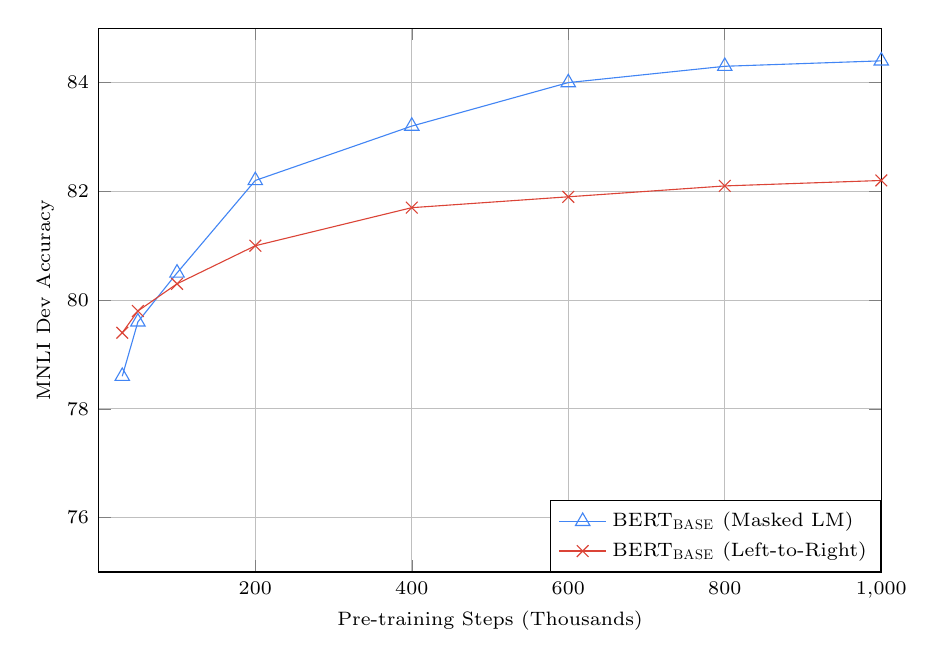
\begin{tikzpicture}
 \begin{axis}[
   width=0.95\columnwidth,
   height=0.7\columnwidth,
   legend cell align=left,
   legend style={at={(1, 0)},anchor=south east,font=\scriptsize},
   mark options={mark size=3},
   font=\scriptsize,
   xmin=0, xmax=1000,
   ymin=75, ymax=85,
   xtick={200,400,600,800,1000},
   ymajorgrids=true,
   xmajorgrids=true,
   xlabel style={yshift=0.5ex,},
   xlabel=Pre-training Steps (Thousands) ,
   ylabel=MNLI Dev Accuracy,
   ylabel style={yshift=-0.5ex,}]
    \addplot[mark=triangle,g-blue] plot coordinates {
      (30, 78.6)
      (50, 79.6)
      (100, 80.5)
      (200, 82.2)
      (400, 83.2)
      (600, 84.0)
      (800, 84.3)
      (1000, 84.4)
    };
    \addlegendentry{\bertbase (Masked LM)}
    \addplot[mark=x,g-red] plot coordinates {
      (30, 79.4)
      (50, 79.8)
      (100, 80.3)
      (200, 81.0)
      (400, 81.7)
      (600, 81.9)
      (800, 82.1)
      (1000, 82.2)
    };
    \addlegendentry{\bertbase (Left-to-Right)}
     \end{axis}
\end{tikzpicture}
\caption{Ablation over number of training steps. This shows the MNLI accuracy after fine-tuning, starting from model parameters that have been pre-trained for $k$ steps. The x-axis is the value of $k$.}
\label{fig:step_abalation}
\end{figure}

\subsection{Feature-based Approach with BERT}
\begin{table}[b]
\centering
 \begin{tabular}{@{}lc@{}}
    \toprule
 Layers & \multicolumn{1}{c}{Dev  F1} \\
    \midrule
Finetune All&	96.4 \\
    \midrule
First Layer (Embeddings)    & 91.0 \\
Second-to-Last Hidden   & 95.6 \\
Last Hidden            & 94.9 \\
Sum Last Four Hidden        & 95.9 \\
Concat Last Four Hidden        & 96.1 \\
Sum All 12 Layers        & 95.5 \\
     \bottomrule
   \end{tabular}
   \caption{Ablation using BERT with a feature-based approach on CoNLL-2003 NER. The activations from the specified layers are combined and fed into a two-layer BiLSTM, without backpropagation to BERT.}
   \label{tab:pretrained_embeddings}    
\end{table}

All of the BERT results presented so far have used the fine-tuning approach, where a simple classification layer is added to the pre-trained model, and all parameters are jointly fine-tuned on a downstream task. However, the feature-based approach, where fixed features are extracted from the pre-trained model, has certain advantages. First, not all NLP tasks can be easily be represented by a Transformer encoder architecture, and therefore require a task-specific model architecture to be added. Second, there are major computational benefits to being able to pre-compute an expensive representation of the training data once and then run many experiments with less expensive models on top of this representation. 

In this section we evaluate how well BERT performs in the feature-based approach by generating ELMo-like pre-trained contextual representations on the CoNLL-2003 NER task. To do this, we use the same input representation as in Section~\ref{sec:ner}, but use the activations from one or more layers {\it without} fine-tuning any parameters of BERT. These contextual embeddings are used as input to a randomly initialized two-layer 768-dimensional BiLSTM before the classification layer.

Results are shown in Table~\ref{tab:pretrained_embeddings}. The best performing method is to concatenate the token representations from the top four hidden layers of the pre-trained Transformer, which is only 0.3 F1 behind fine-tuning the entire model. This demonstrates that BERT is effective for both the fine-tuning and feature-based approaches.


\section{Conclusion}
Recent empirical improvements due to transfer learning with language models have demonstrated that rich, unsupervised pre-training is an integral part of many language understanding systems. In particular, these results enable even low-resource tasks to benefit from very deep unidirectional architectures. Our major contribution is further generalizing these findings to deep \emph{bidirectional} architectures, allowing the same pre-trained model to successfully tackle a broad set of NLP tasks.

While the empirical results are strong, in some cases surpassing human performance, important future work is to investigate the linguistic phenomena that may or may not be captured by BERT.


\bibliographystyle{acl_natbib}
\bibliography{lumiere}

\end{document}
